
\documentclass{article}

\usepackage{amsmath}
\usepackage{amssymb}
\usepackage{amsthm}
\usepackage{amsfonts}
\usepackage{pgfplots}
\usepackage[a4paper,margin=1in]{geometry}

\title{Differential Geometry}
\author{Ciarán Ó hAoláín}

\let\nset\varnothing
\let\ddd\cdots

\newcommand{\sth}{\ \mathrm{s.th\ }}
\renewcommand{\d}{\mathrm{d}}
\newcommand{\N}{\mathbb{N}}
\newcommand{\R}{\mathbb{R}}
\newcommand{\C}{\mathbb{C}}
\newcommand{\dv}[2]{\frac{\d #1}{\d #2}}
\newcommand{\pdv}[2]{\frac{\partial #1}{\partial #2}}
\newcommand{\fdv}[3]{\left.\dv{#1}{#2}\right|_{#3}}
\newcommand{\crit}{\mathrm{Crit}\ }
\newcommand{\im}{\mathrm{Im}\ }	
\newcommand{\abs}[1]{\left|#1\right|}
\newcommand{\osub}{\subset_\mathrm{open}}

\newtheorem{theorem}{Theorem}[section]
\newtheorem{corollary}{Corollary}[theorem]
\newtheorem{lemma}[theorem]{Lemma}
\theoremstyle{definition}
\newtheorem{definition}{Definition}[section]
\theoremstyle{remark}
\theoremstyle{example}
\newtheorem*{remark}{Remark}
\newtheorem*{example}{Example}


\begin{document}
	\maketitle
	
	\section{Tutorial (19.09.30)}
	\begin{definition}
		A curve in $\R^3$ is a smooth function $\alpha:I \to \R^3$.\\
		Here $I=[a,b]$, an interval in $\R$.\\
		\[ \alpha(t) = (\alpha_1(t), \alpha_2(t), \alpha_3(t))  \]\\
		where $\alpha_i : I \to \R$ is a smooth $C^\infty$ for each $i$.
		\begin{remark}
			Technically, some regard the curve as the \textbf{image} of the parameterisation of the map $I \to \R^3$.
		\end{remark}
	\end{definition}

	\begin{definition}
		Given a curve $\alpha:I \to \R^3$, the \textbf{velocity vector} of $\alpha$ at a time $t_0 \in I$ is the tangent vector \[\alpha'(t_0\alpha(t_0)) = (\alpha_1'(t_0), \alpha_2'(t_0), \alpha_3(t_0))_{\alpha(t_0)} \in I_\alpha(t_0)\R^3 \]
	\end{definition}
	\begin{remark}
		Henceforth we supress the subscript notation and write $\alpha'(t_0):= \alpha'(t_0)_{\alpha(t_0)}$
	\end{remark}

	\begin{definition}
		$f: \R^3 \to \R$, a function is smooth ($C^\infty$) if at all points $p \in \R^3$, all partial derivatives of $f$ of all orders exist and are continuous.\\
		$C^\infty(\R^3):=$ ring (under usual additions, multiplications) of all smooth functions $\R^3 \to \R$.
	\end{definition}

	\begin{definition}
		Let $\vec{v_p} \leftarrow T \R^3 $ be some tangent vector and let $f:\R^3 \to \R$ be a smooth function.\\
		The \textbf{directional derivative} of $f$ at $p$ in the direction $v$ (of $f$ at $v_p$) is given by: \[\d f_p(\vec{v}) = D_{\vec{v_p}(f)} := \frac{\d}{\d t}_{t=0}f(p+t \vec{v})\]
	\end{definition}

	Common notation: $v_p[f]:=D_{v_p}(f)=\d f_p(\vec{v})$
	\begin{example}
		$f(x,y,z) = x^2yz+e^xz\\
		\vec{v_p}=(1,-1,0)_(1,2,1)\\
		$ Compute $\vec{v_p}[f].\\
		p+t\vec{v}=(1,2,1) + t(1,-1,0) = (1+t, 2-t, 1).\\
		f(p+t\vec{v}) = (1+t)^2(2-t)(1)+e^{1+t}\\
		= (1+2t+t^2)(2-t)+e^{1+t}\\
		= (2 + 4t + 2t^2) - t - 2t^2 - t^3 + e^{1+t}\\
		= 2 + 3t-t^3 + e^{1+t}$
	\end{example}

	\begin{definition}[Basic Properties]
		Assume fixed $v+p \in T \R^3$ and $f,g \in C^\infty(\R^3)$.
		\begin{enumerate}
			\item $v_p[f+g] = v_p[f] + v_p[g]$
			\item $v_p[cf] = cv_p[f], c$ constant. (1,2 - linearity)
			\item $v_p[fg]=(v_p[f])g(p) + f(p).v_p[g]$ (Leibniz)
		\end{enumerate}
	\end{definition}

	\begin{definition}
		A (tangent) vector field to $\R^3$ is a function \begin{align*}
			 X: \R^3 & \to & T \R^3\\
			  p & \mapsto & (X_1(p), X_2(p), X_3(p))_{(p)}\\
		\end{align*}
		with each $X_i:\R^3 \to \R$ smooth.
	\end{definition}

	Observe that for each $p \in \R^3$, \[ X(p) \in T_p\R^3 \]
	Further abuse of notation: drop subscript $p$.\\
	\[ X(p) = (X_1(p), X_2 \ddd )_{(p)} \]

	$\Gamma T \R^3 $ is the set of all tangent vector fields to $\R^3$\\
	$\ \in \Gamma T \R^3 , f \in C^\infty (\R^3)\\$
	\begin{definition}
	Define $X[f]$ to be the function $\R^3 \to \R$, $p \mapsto X(p)[f]$.Some properties:
	\begin{enumerate}
		\item $X,Y \in \Gamma T \R^3$
		\item $(X+_c Y)$
	\end{enumerate}
	\end{definition}

	\section{Lecture 3 (2019.10.02)}
	$C^\infty(\R^3) :=$ smooth functions $\R^3 \to \R$.\\
	$X \in \Gamma T \R^3 := $ vector fields on $\R^3$\\
	\begin{align*}
		X:\R^3 \to & T \R^3\\
		p \mapsto & X(P)\in T_p\R^3
	\end{align*}
	$X(p) = (X_1(p),X_2(p),X_3(p))_p$\\
	$X_i:\R^3 \to \R$ smooth functions in $p$, $x_i \in C^\infty(\R^3)$.\\
	Recall, $X,Y \in \Gamma T \R^3, f \in C^\infty(\R^3)$\\
	\begin{enumerate}
		\item $X+fY \in \Gamma T \R^3$
		\item $X \times Y \in \Gamma T \R^3$
		\item $X.Y \in C^\infty(\R^3)$
	\end{enumerate}

	\begin{definition}[Gradient]
		Given $f \in C^\infty(\R^3)$, we define the \textbf{gradient} of $f$, written grad$f$ or $\nabla f$ as 
		\[ \nabla f = \begin{pmatrix}
			\pdv{f}{x} (p) & \pdv{f}{y} (p) & \pdv{f}{z} (p) 
		\end{pmatrix}\]
		$\nabla f \in \Gamma  T \R^3$, a vector field arising from dot product. Essentially $\nabla f$ is the vector field pointing in the direction of the greatest rate of change of $f$.\\
		Formally, \[ \begin{pmatrix}
			\nabla = \pdv{}{x} (p) & \pdv{}{y} (p) & \pdv{}{z}
		\end{pmatrix} \]
	\end{definition}

	Consider $f \in C^\infty (\R^3) $, $v_p \in T \R^3$\\
	Recall $v_p[f] = \dv{}{t}|_{t=0}f(p+t \vec{v})$\\
	Fact: Replace $t \mapsto p+t \vec{v}$ with any curve: \[ t \mapsto \alpha(t)=(\alpha_1(t) \ddd)\] satisfying $\alpha'(0)=v_p$, and $\alpha(0)=p$.\\
	\[ v_p[f]:=\dv{}{t}|_{t=0} f(p+t \vec{v}) = \dv{}{t}|_{t=0} f(\alpha(t))\]\\
	\begin{align*}
		v_p[f]=\dv{}{t}|_{t=0} f(\alpha(t)) & = \pdv{f}{x}(\overbrace{\alpha(0)}^p)\alpha_1'(0) + \pdv{f}{y}(\alpha(0)^p)\alpha_2'(0) + \pdv{f}{z}(\alpha(0))\alpha_3'(0)\\
		& = \pdv{f}{x}(p)v_1 + \pdv{f}{y}(p)v_2 + \pdv{f}{z}(p)v_3\\
		& = \nabla f(p) . \vec{v}
	\end{align*}
	
	Compute now the case when $\vec{v}$ is unit $(|\vec{v}|=1)$.\\
	It is common to compute the directional derivative in this case only.\\
	\begin{align*}
		v_p[f]=\nabla f(p).\vec{v} & = |\nabla f(p)| . |\vec{v}| \cos \theta\\
		& = |\nabla f(p)| \cos \theta
	\end{align*}
	This is maximal when $\theta=0$, i.e. when $\vec{v}$ points in the direction of $\nabla f(p)$.\\
	\begin{example}
		Did some drawn examples (f2.2)
	\end{example}

	\begin{definition}
		Given $f \in C^\infty(\R^3), c \in \R$\\
		Let $\gamma : (-\epsilon,\epsilon) \to \R^3$ be a curve satisfying \[ f(\gamma(t)) = c \qquad \forall t \in (-\epsilon,\epsilon)\]
		Set $p:= \gamma(0)$ and note the image of $\gamma$ lies entirely on the level set $f^{-1}(c)$ (F.2.3)\\
		Notice that \[ v_p[f]=\left.\dv{}{t}\right|_{t=0}(f(\gamma(t)))=\nabla f(p).\vec{v_p} \]
		But $f(\gamma(t))=c,$ contstant, $\forall t \in (-\epsilon,\epsilon)$\\
		Thus $\gamma f(p),v_p=0, $ hence $\nabla F(p) \perp \vec{v}.\\$
		Little more..
	\end{definition}

	In th case when $|\vec{v}|=1$ deduce that $v_p[f]$ is maximal when $\vec{v}$ is parallel to $\nabla f(p)$.\\
	Secondly, $\forall p \in \R^3$ set $c=f(p)$.\\
	$\nabla f(p) \perp$ to $f^{-1}(c)$ at $p$.\\
	$f^{-1}(c)=\{(x,y,z) \in \R^3 : f(x,y,z)=c\}$ (level set at $c$).
	
	\begin{remark}
		\begin{align*}
		 C^\infty(X,Y)& := \{f : X \to Y \ \mathrm{smooth} \}\\
		 C^\infty(X) &:= \{f : X \to \R \  \mathrm{smooth} \}
		\end{align*}
	\end{remark}
	
	\begin{definition}
		Given $f \in C^\infty(\R^3)$, a point $p \in \R^3$ is a critical point of $f$ if $\nabla f(p)=(0,0,0)$.
		Otherwise, $p \in \R^3$ is called a regular point of $f$.\\
		\[\mathrm{Crit}\ f := \{p \in \R^3:\nabla f(p)=\vec{0}\} \]
		is the set of critical points of $f$.
	\end{definition}

	\begin{example}
		\begin{align*}
			f(x,y,z) & = -x^2+y^2+z^2\\
			\nabla f & = (-2x,2y,2z)\\
			\crit f & = \{(0,0,0)\}
		\end{align*}
		As $f(0,0,0)=0$, we consider $f^{-1}(0)$ to be a "critical" level set.
	\end{example}
	
	\pagebreak

	\section*{Lecture 5 (19.10.9)}
	Recall $C^\infty(\R^3)$ is the smooth functions $\R^3 \to \R$\\
	$X \in \Gamma (T \R^3)$ is the smooth vector fields on $\R^3$\\
	$X=(X_1,X_2,X_3)$ where $X_i \in C^\infty(\R^3) \ \forall i$\\
	$E_1 \ddd E_2 $ are the constant vector fields on $\R^3$.\\
	$\forall p \in \R^3, \{E_1(p),E_2(p),E_3(p)\}$ is the standard (orthonormal) basis for $T_p\R^3 \cong \R^3$.\\
	Thus we sometimes write \[X=X_1E_1+X_2E_2+X_3E_3 = \sum_{i=1}^{3}X_iE_i \]\\
	The triple of vector fields $\{E_1,E_2,E_3\}$ is an example of an (orthonormal) \textbf{frame field} on $\R^3$.\\
	More generally an (orthonormal) \textbf{frame field} on $\R^3$ is a triple of vector fields \[\{X,Y,Z\} \sth \forall p \in \R^3, \{X(p),Y(p),Z(p)\}\] is an (orthonormal) \textbf{basis} for $T_p\R^3$.\\
	Finally, recall \[X,y \in \Gamma T \R^3, f \in C^\infty (\R^3) \]
	\begin{enumerate}
		\item $X.Y \in C^\infty (\R^3)$
		\begin{align*}
			X.Y:\R^3 & \to \R\\
			p & \mapsto X(p).Y(p)
		\end{align*}
		\item $X \times Y \in \Gamma T \R^3 \qquad (X \times Y)(p) := X(p) \times Y(p)$
		\item $X + fY \in \Gamma T \R^3$
		\[ (X+fY)(p) := X(p) + \underbrace{f(p)}_\mathrm{scalar} Y(p) \]
	\end{enumerate}

	\subsection{Curves in $\R^3$}
	Recall $\alpha:I \to \R^3, I=[a,b] \subset \R$ is a \textbf{smooth curve} provided each of $\alpha_i(t)$ is a smooth function where $\alpha(t)=(\alpha_1(t),\alpha_2(t), \alpha_3(t))$.
	
	\begin{remark}
		Some people like to think of the \textbf{curve} as the \textbf{image} of $\alpha$, where $\alpha$ is just one of many parameterisations.
	\end{remark}

	\begin{definition}
		A curve is said to be a \textbf{regular}, provided $|\alpha'(t)|>0\  \forall t$
	\end{definition}

	\begin{remark}
		Recall $\alpha'(t)=(\alpha'_1(t),\alpha'_2(t), \alpha'_3(t))$ is the \textbf{velocity vector field} to $\alpha$.
	\end{remark}

	\begin{definition}
		A curve $\alpha : I \to \R^3$ is said to be \textbf{arc-length parameterised, or unit speed} if $|\alpha'_t|=1\ \forall t \in [a,b]$.
	\end{definition}

	\begin{theorem}
		Any regular curve $\alpha : I \to \R^3$ can be reparameterised as a unit speed curve $tilde{\alpha}:\tilde{I} \to \R^3$ where $\im \alpha = \im \tilde{\alpha}$
	\end{theorem}

	\begin{proof}
		Given $\alpha : [a,b] \to \R^3$ a regular curve with $\alpha(t)=(\alpha_1(t),\alpha_2(t),\alpha_3(t))$.\\
		Define \[s(t) := \int_{a}^{t}|\alpha'(u) |\d u \]
		where $|\alpha'(u)|$ is the speed at time $u$.\\
		Notice $0=s(a) \leq s(t) \leq L=s(b)$.\\
		Notice $s'(t)=|\alpha'(t)| > 0$.\\
		Thus $s(t)$ is invertible. Call the inverse $t(s)$.\\
		Define $\tilde{\alpha}(s):=\alpha(t(s))$.\\
		This gives a curve: $\tilde{\alpha}:\underbrace{[0,L]}_{\tilde{I}} \to \R^3$\\
		Moreover,
		\begin{align*}
			\tilde{\alpha'}(s) & =\underbrace{\alpha'(t)}_\mathrm{vec}\underbrace{(t'(s)}_\mathrm{scalar})\\
			\Gamma & = (\alpha'_1(t),t'(s),\alpha'_2(t)t'(s),\alpha'_3(t)t'(s))\\
			& = \alpha'(t)\frac{1}{s'(t)}\\
			& = \frac{\alpha'(t)}{|\alpha'(t)|}
		\end{align*}
		which is unit length.
	\end{proof}

	\begin{example}[Spiral staircase]
		\begin{align*}
			\alpha(t)&=(\cos t, \sin t, t) & t \in [0, 2\pi]\\
			\alpha'(t)&=(-\sin t,\cos t, 1) & \alpha'(t) \neq \vec{0}\ \forall t\\
			|\alpha'(u)|&=\sqrt{(-\sin u)^2 + (\cos u)^2 + 1} & = \sqrt{2}\\
			s(t)&=\int_{0}^{t}\sqrt{2}\ \d u
		\end{align*}
		\textbf{Need end of example/computation here.}
	\end{example}

	\section*{Lecture 6 (19.10.10)}
	\section{Curvature of 1-dimensional curves}
	Set up $\alpha:I \to \R^3$ regular curve.\\
	Recall $\alpha':I \to T \R^3$ is the velocity vector field to $\alpha$.\\
	Differentiating gives $\alpha''=(\alpha')':I \to T \R^3$ to be the accelerating vector field.
	In general, a vector field along $\alpha$ is a smooth map $X : I \to T \R^3$ satisfying $X(T) \in T_{\alpha(t)} \R^3$ (not necessarily tangent to the curve).
	\begin{definition}[Some properties of vector fields on $\alpha$]
		Given $X,Y:I \to T\R^3,f:I \to \R$ smooth function.
		\begin{enumerate}
			\item $X+f$ is a vector field on $\alpha$.\\
			\item $X.Y:I \to \R,t \mapsto X(t).Y(t)$ is a smooth real valued function
			\item $X \times Y$ is a vector field on $\alpha$, ($(X \times Y)(t):=X(t)\times Y(t)$)
			\item $X':I \to T \R^3$ is a vector field
			\item $(X+cY)'=X'+cY'$, $c$ is a constant
			\item $(fX)'(t)=f'(t)X(t)+f(t)X'(t)$
		\end{enumerate}
	\end{definition}
	Assume $\alpha$ is a constant speed curve (i.e. $\alpha'\equiv\vec{c}$ constant)\\
	Fact: $\alpha$ is a constant curve ($\im \alpha = $ a point) $\iff \alpha' \equiv \vec{0}$\\
	Fact: A straight line in $\R^3 \iff \alpha$ has $\alpha''\equiv\vec{0}$.
	
	Goal: measure curvature of $\alpha$ independently from the parameterisation.\\
	Henceforth assume $\alpha$ is unit speed parameterised.\\
	Rename as $\beta(s)$ (unit speed curve).
	
	$|\beta'(s)|=I \forall s \in I$.
	Define $T(s):=\beta'(s)$ (unit tangent vector field to $\beta$)\\
	$b-a=$length of $\beta$\\
	What is $T'$? $T'-(\beta')'$\\
	Notice $T.T\equiv 1$ constantly.\\
	$(T.T)'=T.T'+T'T=2T.T'
	=-$ since ($1'=0$)\\
	So $T \perp T'$.
	
	Define the curvature to $\beta$ at $s$ as $\kappa(s):=|T'(s)|=|\beta''(s)|$.
	
	\begin{example}
		\begin{align*}
			\alpha(t)&=(\cos t, \sin t, t) & t \in [0,2 \pi]\\
			\beta(s) &=\left(\cos \frac{s}{\sqrt{2}},\sin \frac{s}{\sqrt{2}}, \frac{s}{\sqrt{2}} \right) & s \in [0,\sqrt{2} 2 \pi]\\
			\beta'(s) & = \left( \frac{-1}{\sqrt{2}} \sin \frac{5}{\sqrt{2}},\frac{1}{\sqrt{2}} \cos \frac{5}{\sqrt{2}} ,\frac{1}{\sqrt{2}}\right)
		\end{align*}
	\end{example}
	\[ \kappa(s)=|\beta''(s)|=\sqrt{(-\tfrac{1}{2})^2}=\tfrac{1}{2} \]
	An arbitrary unit. soeed curve $\beta$ may have straight line segments (i.e. with $\kappa \equiv 0$)\\
	Assume for now that $\beta:I \to \R^3$ is a curve with $\kappa(s)>0\ \forall s \in I$.\\
	Now $T'(s) \neq (0,0,0)\ \forall s \in I$.\\
	Define $N$ a vector field on $\beta$, by \[N(S)=\frac{T'(S)}{|T'(S)|}=\frac{T'(S)}{\kappa(s)}\]
	Notice $T'(s)=\kappa(s)N$.
	Finally $\beta:= T \times N$.\\
	The three:
	$T:=$ tangent vector field\\
	$N:=$ normal vector field\\
	$\beta :=$ binormal vector field\\
	Form a \textbf{Frenet Frame}
	
	
	\pagebreak
	\section*{Lecture 7 (19.10.16)}
	\begin{definition}[Frenet Frames]
		Given a unit speed curve
		\begin{align*}
		\beta : I &\to \R^3\\
		s & \mapsto \beta(s)=(\beta_1(s),\beta_2(s),\beta_3(s))
		\end{align*}
		Tangent vector $T(s)=\beta'(s)\qquad \kappa(s):=|\beta''(s)|$ curvature.\\
		Recall $\beta''(s).T(s)=0$\\
		Assume for now $\kappa(s)>0\ \forall s$\\
		Now can define \begin{align*}
		N(s)&:=\frac{\beta''(s)}{\kappa(s)}&\mathrm{(normal)}\\
		\beta(S)&:=T(s) \times N(s) & \mathrm{(binormal)}
		\end{align*}
		The triple $\{T,N,\beta\}$ is called the Frenet Frame field.\\
		The triple at $s, \{T(s),N(s),\beta(s)\}$ is called the Frenet Frame (an orthonormal basis for $T_{\beta(s)}\R^3)$
	\end{definition}
	We will now derive what are known as the Frenet Formulae\\(i.e. compute $T',N',\beta'$)
	\begin{align*}
		T'&=\beta''=|\beta''|\frac{\beta''}{|\beta''|}=\kappa N\\
		(\beta . T)'&=0\\
		\beta . T & = -\beta . T' = - \beta . (\kappa N) = 0\\
		\beta . \beta &= 0 & (\beta . \beta)'=1'=0\\
		2\beta.\beta'&=0 & \mathrm{Leibnix}
	\end{align*}
	Now we know that $\beta' \perp T,  \beta' \perp N$.\\
	Thus $\beta'$ is a scalar multiple of $N$.\\
	i.e. $\forall s\ \beta'(s)=-\tau(s)N(s)$ for some $\tau(s)$.\\
	We call the smoothly varying scalar function $\tau(s)$, the \textbf{torsion} of $\beta$ at $s$.\\
	Finally \[N'=(N'.T)T+(N'.N)N+(N'.\beta)\beta \]
	$N'.T=?$
	\begin{align*}
		N.T & = 0\\
		N'T & = -N.T'=-N.(\kappa N)=-\kappa
	\end{align*}
	$N'.N=?$
	\begin{align*}
		N.N&=0\\
		N'.N&=-(N'.N)=0
	\end{align*}
	$N'.\beta=?$
	\begin{align*}
		N.\beta&=0\\
		N'.\beta&=-N.\beta'\\
		&=-N.(-\tau N)\\
		&= \tau
	\end{align*}
	Option: Define as $\beta'=-\tau N$\\
	Define torsion as $-\beta'N$.
	In conclusion we have \[\begin{matrix}
		T'&=&& \kappa N\\
		N'&=&-\kappa T& & \tau B\\
		\beta' & =& & -\tau N
	\end{matrix}\]\\
	Assume $0 \in I$ (could be any $s_0 \in I$)\\
	Near 0, \[\beta(s)=\beta(0)+s \beta'(0)+ \frac{s^2}{2}\beta''(0) + \frac{s^3}{6}\beta'''(0) + \ddd \]\\
	$\beta'(0)=T(0)$\\
	$\beta''(0)=T'(0)=\kappa(0)N(0)$
	\begin{align*}
		\beta'''(0)&=(T')'(0)\\
		&=(\kappa N)'(0)\\
		& = \kappa(0) N'(0)+\kappa'(0)N(0)\\
		& = \kappa(0) \left[-\kappa(0)T(0)+\tau(0)\beta(0)\right]+\kappa;(0)N(0)
	\end{align*}
	Thus \[\beta'''(0)=-\kappa(0)^2T(0)_\kappa(0)\tau(0)\beta(0)+\kappa'(0)N(0)\]
	\begin{align*}
		\beta(s)&=\beta(0)+sT(0)+\frac{s^2}{2}\kappa(0)N(0)+\frac{s^3}{6}(-\kappa(0)^2T(0)+\kappa(0)\tau(0)\beta(0)+\kappa'(0)N(0)) + \mathrm{h.o.t}\\
		&=\beta(0)+\left[s-\kappa(0)^2\frac{s^3}{6}\right]T(0)+\left[\frac{s^2}{2}\kappa(0)+\frac{s^3}{6}\kappa'(0)\right]N(0)+\frac{s^3}{6}\kappa(0)T(0)\beta(0)+\mathrm{h.o.t}
	\end{align*}
	Fact: $\beta$ is a planar curve $\iff \tau \equiv 0$\\
	Idea: From Taylor expansion above, all h.o.t contain $\tau$ or its derivatives.\\
	Thus $\tau \equiv 0$ makes $\beta(s)$ lie a plane spanned by $T(0),N(0)$.
	
	\section*{Lecture}
	\textbf{Missing some stuff}
	Thus $\gamma(s)=\vec{c}$ constant.\\
	\begin{align*}
		\d_{Euc}(\beta(s), \vec{c})&=\d_{Euc}(\beta(s),\beta(s)+\frac{1}{\kappa}N(s))\\
		&=\left|\frac{1}{\kappa}N(s)\right|\\
		&=\frac{1}{\kappa}\ \mathrm{(constant)}
	\end{align*}
	
	Given a general curve  $\beta : I \to \R^3$ (unit sp. $\kappa(s)>0\ \forall s \in I$) (possibly $\tau \neq 0$)\\
	Fact: For any $s_0 \in I$ (open), $\exists$ a unique circle, parameterised by $\gamma:[-\pi,\pi]\to \R^3 \sth$
	\begin{align*}
		\gamma(0)&=\beta(s_0)\\
		\gamma'(0)=\beta'(s_0)\\
		\gamma''(0)=\beta''(s_0)
	\end{align*}
	This circle is the "best fitting circle" to $\beta$ at $s_0$.\\
	It is called the \textbf{osculating circle} to $\beta$ at $s_0$, and it lies on the plane spanned by $T(s_0)$ and $N(s_0)$. It has centre $z=\beta(s_0)+\frac{1}{\kappa(s_0)}N(s_0)$ and radius $\frac{1}{\kappa(s_0)}$
	
	\begin{definition}[Spherical Curves]
		A curve $\beta:I\to\R^3$ is said to be spherical if \[\abs{\beta(s)}=r>0\  \mathrm{constant}\qquad \forall s\]
	\end{definition}
	\begin{remark}[Notation]
		\[S^2(r):=\{(x,y,z) \in \R^3:x^2+y^2+z^2=r^2\} \]
		i.e. $\im \beta \subset S^2(r)$
	\end{remark}

	\begin{theorem}
		A unit speed curve $\beta:I\to S^2(r) \subset \R^3$ has curvature function satisfying \[\kappa(s)\geq \frac{1}{r}\] 
	\end{theorem}
	\begin{proof}
		Observe $\beta(s).\beta(s)=r^2$ constant.\\
		$\beta'(s).\beta(s)=0$.
		i.e. \begin{align*}
			T.\beta&=0\\
			T'.\beta+\beta'.T&=0\\
			\kappa N . \beta &=-T.T=-1\\
			\abs{N.\beta} &=\frac{1}{\kappa}
		\end{align*}
		But $\abs{\beta.N}\leq \abs{\beta} \abs{N} = r.1=r$.
	\end{proof}

	\section*{Tutorial 2}
	\begin{align*}
		f_t(x,y,z)&=z^3+tz-x^2+y^2 & t=-1,0,1\\
		\nabla f_t &= (-2x,2y,3z^2+t)\\
		\crit f_t &=\left\{ (0,0,z) \left| z=\pm \sqrt{\frac{-t}{3}}\right. \right\}
	\end{align*}
	
	\section{Surfaces}
	PREVIEW:\\
	Idea: A surface is locally topologically equivalent to $\R^3$. We have a homeomorphism (cts. bijection with cts. inverse)
	
	\begin{remark}
		Topology: Things can be topologically the same, but geometrically different.
	\end{remark}

	Non-example: \[\{(x,y,z)\in\R^3 :-x^2+y^2+z^2=0 \}\]
	
	\section*{Lecture 19.10.23}
	$U \subset_\mathrm{open} \R^n$\\
	\begin{align*}
		F:U&\to \R^m\\
		(x)....
	\end{align*}
	$p \in U \subset_\mathrm{open}\R^n\\
	T_pU=T_p\R^n$\\
	\begin{definition}[Derivative map]
		The deriviative map of $F$ at $p$ is the linear map \[DF_p:T_p... \] defined \[ DF_p(\vec{v}) = \fdv{}{t}{t=0}F(p+t\vec{v}) \]
		Notice that \[ DF_p(\vec{v})=(v_p[F_1], v_p[F_2],\ddd,v_p[F_m])\]
	\end{definition}
	\begin{example}
		\begin{align*}
			F:\R^2 &\to \R^2\\
			(x,y) & \mapsto (x^2-y^2,2xy)
		\end{align*}
		\[DF_p= \begin{bmatrix}
			2x&-2y\\
			2y & 2x
		\end{bmatrix}_p = \begin{bmatrix}
		2p_1&-2p_2\\
		2p_2 & 2p_1
		\end{bmatrix} \]
	\end{example}
	\begin{definition}
		A smooth map $F:U\subset_\mathrm{open}\R^n \to \R^m$ is said to be an \textbf{immersion} if $\forall p \in U$, the derivative $DF_p:T_p\R^n \to T_{F(p)}\R^m$ is injective (has rank $n$).\\
		$F$ is said to be a submersion if $DF_p$ is surjective $\forall p \in U$ (rank $m$).
	\end{definition}
	\begin{example}
		\begin{align*}
			\alpha:\R &\to \R^2\\
			t & \mapsto (\cos t, \sin t)
		\end{align*}
		is an immersion (not injective).
	\end{example}
	\begin{example}
		\begin{align*}
			F:\R^2 & \to \R^3\\
			(\phi, \theta) & \mapsto \begin{bmatrix}
				(2 + \cos \phi) \cos \phi\\
				(2 + \cos \phi) \sin \phi\\
				\sin \phi
			\end{bmatrix}
		\end{align*}
		Check that this is an immersion (not injective).
	\end{example}
	\begin{example}
		\begin{align*}
			F:\R^3 \setminus \{0\} & \to \R\\
			(x,y,z) & \to x^2+y^2+z^2
		\end{align*}
		(submersion)
	\end{example}

	\begin{definition}[Diffeomorphism]
		$U\subset_\mathrm{open}, V \subset_\mathrm{open}\R^m$\\
		\[F:U \to V\] is a \textbf{diffeomorphism} if $F$ is smooth, bijective and has a smooth inverse.
	\end{definition}
	\begin{example}
		Non-example: \begin{align*}
			\R & \to \R\\
			x & \mapsto x^3
		\end{align*}
		is not a diffeomorphism as $x \mapsto x^{\frac{1}{3}}$ is not smooth at 0.
	\end{example}

	FACT: A diffeomorphism is both an immersion and a submersion.\\
	Partial converse: Inverse Function Theorem
	\begin{theorem}[Inverse Function Theorem]
		Suppose $F:U \subset_\mathrm{open} \R^n \to \R^n$ is an immersion at $p \in U$.\\
		(i.e. $\det(DF_p) \neq 0$).\\
		THen $\exists \ nbds\ A \subset U$ and $B \subset \R^n$ with $p \in A, F(p) \in B$ os that $F |_A:A \to B$ is a diffeomorphism.
	\end{theorem}

	\begin{definition}
		Let $M \subset \R^3$ be a subset.\\
		An open neightbourhood of $p \in M$ in $M$ is a subset $V \subset M$ with $p \in V \sth V=M \cap U$ for some open set $U \subset \R^3$.
	\end{definition}

	\begin{definition}
		$M \subset \R^3$ is a surface if $\forall p \in M \exists$ a neighbourhood $V$ in $M$ with $p \in M$, and a map $\phi$ from an open set $U \subset \R^2, \phi:U \to V$ which is a diffeomorphism.
	\end{definition}

	\section*{Lecture (2019.10.24)}
	$U \osub \R^n$\\
	$F:U \to \R^m$ smooth if all partial derivatives of all component functions exist and are cts.
	\begin{remark}[Technical point]
		$X \subset \R^n$ (not necessarily open)\\
		$F:X \to \R^m$ smooth if $\exists$ an "extension"\\
		$\tilde{F}:Y \to_\mathrm{smooth} \R^m$ when $Y \osub \R^n$, $X \subset Y$ and $\tilde{F}|_x=F$.\\
		Given $X_1 \in \R^n, X_2 \subset \R^m$ sets, $F:X_1 \to X_2$ is a diffeomorphism if $F$ smooth, bijective and with smooth inverse.
	\end{remark}

	\begin{definition}[Surface]
		$M \subset \R^3$ is a surface if $\forall p \in M, \exists $ neighbourhood $U \subset M, p \in U $ and a neighbourhood $V \subset \R^2$ along with a diffeomorphism $\varphi : U \to V$.
	\end{definition}

	\section*{Tutorial 2019.11.11}
	$\alpha$ curve, $\kappa > 0$ and $\tau \neq 0$ always.\\
	Notation: $\rho = \frac{1}{k}$ and $\sigma = \frac{1}{\sigma}$\\
	\textbf{Claim:} If $\alpha$ lies on a sphere of radius $r$ centered at $c \in \R$, then \begin{align*}
		\alpha - c &= - \rho N - \rho ' \sigma B\\
		(\alpha-c) \cdot (\alpha - c) = r^2\\
		2T \cdot (\alpha - c) & = 0  & \dv{}{t}\\
		T \cdot \alpha' + (\alpha-c) \cdot T' &= 0 & \dv{}{t}\\
		T\cdot T + (\alpha - c) \cdot T' & = 0\\
		(\alpha-c).T'&=-1\\
		(\alpha-c) \cdot (\kappa N) & = -1\\
		(\alpha-c ) \cdot N &= -\frac{1}{\kappa} = - \rhd
	\end{align*}
	Returning to $(\alpha-c)\cdot T'=-1$:
	\begin{align*}
		T\cdot T' + (\alpha-c) \cdot (T')' & = 0 & \dv{}{t}\\
		T \cdot (\kappa N) + (\alpha -c )\cdot [\kappa N]' & = 0\\
		0 + (\alpha -c )[\kappa'N+\kappa N'] & = 0\\
		(\alpha - c)[\kappa'N + \kappa(-\kappa T+\tau B)] & = 0\\
		(\alpha - c)[\kappa'N-\kappa'T+\kappa\tau B] & = 0\\
		\kappa'((\alpha-c)\cdot N) + \kappa \tau (\alpha - c) \cdot B & = 0\\
		(\alpha - c)\cdot B &= \frac{\kappa'\rho}{\kappa \tau}
	\end{align*}
	\begin{align*}
		(\alpha - c)&=((\alpha - c) \cdot T) T + ((\alpha - c) \cdot N) N + ((\alpha - c)\cdot B) B\\
		& = (0)T + (-\rho N) + (\frac{\kappa' \rho}{\kappa \tau}) B\\
		& = -\rho N - \left(\frac{\kappa'}{\kappa^2}\right)\sigma\\
		& = -\rho N - \rho' \sigma B
	\end{align*}
	
	\begin{align*}
		(\alpha - c) \cdot(\alpha - c)&=r^2\\
		(-\rho N - \rho'\sigma B)\cdot(-\rho N - \rho' \sigma B) &= r^2\\
		\rho^2+(p')^2\rho^2&=r^2\\
		r=\sqrt{\rho^2+(\rho'r)^2}
	\end{align*}
	
	And finally \begin{align*}
		(\alpha - c)& = -\rho N - \rho' \sigma B\\
		\alpha + \rho N + rho' \sigma B &= 0\\
		T+\rho N' + \rho' N + \dv{}{t}(\rho' \sigma) B + \rho' \sigma B' &= 0 & \dv{}{t}\\
		T + \rho[-\kappa T + \tau B] + \rho' N + \dv{}{t}(\rho' \sigma) B + \rho' \sigma(- \tau N) & = 0\\
		\overbrace{T+\frac{1}{\kappa}\left(- \kappa \right) T}^{=0} + \rho \tau B + \rho'N+
	\end{align*}
	\pagebreak
	\section*{Lecture 2019.11.13}
	$p \in M \subset \R^3$ surface\\
	$T_pM$ denotes the tangent space (plane) to $M$ at $p$.\\
	\begin{remark}
		Recall $\R^3 \cong T_p\R^3$ tangent space to $\R^3$ at $p \in \R^3$.\\
		$\R^3 \times \R^3 \cong T\R^3: \bigcup_{p \in \R^3} T_p \R^3$ rangent bundle to $\R^3$.\\
		A smooth map \begin{align*}
			X:\R^3 & \to T\R^3\\
			p & \mapsto v_p
		\end{align*}
		(note $X(p) \in T_p\R^3 \subset T\R^3$)
		is called a \textbf{vector field}.\\
		For any subset $A \subset \R^3$, we can define a vector field on $A$ by a \textbf{smooth} map \begin{align*}
			X:A & \to  T\R^3\\
			p & \mapsto v_p \in T_p\R^3, p \in A
		\end{align*}
		$\Gamma T \R^3$ is the set of vector fields on $\R^3$.
	\end{remark}

	\begin{definition}[Vector field on $M$]
		A vector field on $M$ is a smooth map \begin{align*}
		X:M & \to T \R^3\\
		p & \mapsto X(p) \in T_p \R^3
		\end{align*}
	\end{definition}
	
	\begin{definition}[Tangent Vector Field to $M$]
		A Tangent Vector Field to $M$ is a vector field $X:M \to T\R^3 \sth X(p) \in T_pM \subset T_p\R^3, \forall p \in M$.
	\end{definition}

	\begin{definition}[Tangent bundle to $M$]
		\[TM:=\bigcup_{p \in M}T_pM \] is the tangent bundle to $M$.
	\end{definition}

	\begin{definition}
		A tangent vector field to $M$ is a smooth map \begin{align*}
		X:M & \to TM\\
		p&\mapsto X(p) \in T_pM
	\end{align*}
	\end{definition}

	\begin{remark}
		Recall, earlier we noted \[T\R^3 \cong \R^3 \times \R^3 \]
		\textbf{Fact:} This analogous statement for $M$ is often false.\\
		e.g. \[TS^2 \ncong S^2 \times \R^2 \]
		In fact, any single tangent vector field on $S^2$ must have vanishing points (i.e. points $p \sth X(p)=\vec{0} \in T_pM$).\\
		This fact is called \textbf{The Hairy Ball Theorem}. Can we comb the tangent vector (hairs) to avoid (cowlicks) vanishing points? \textbf{No.}\\
		However $T^2$ does have non-vanishing tangent vector fields.\\
		In fact, can find 2 everywhere linearly independent such tangent vector fields on $T^2$ thus showing $T(T^2) \cong T^2 \times \R^2$\\
		Connected sum of $g$ tori: $\Gamma \sum_g \ncong \sum_g \times \R^2, g \geq 2$.
	\end{remark}
\pagebreak
	\begin{definition}
		$M \subset \R^3$ a surface.\\
		Assume we have a polyganalisation of $M$.\\
		$v=\#$ vertices, $e=\#$ edges, $f=\#$ faces.\\
		Euler characteristic \textbf{MISSING}\\
		Sphere is 1-1+2?
	\end{definition}
	\textbf{Fact:} $X(T^2)=0$\\
	$X(\sum_g)=2-2g$.\\
	\\
	Back to the tangent vector fields:\\
	Can associate a number $\pm 1$ to each vanishing point. Outwards is 1 (source), inwards is +1 (sink), saddle is -1.\\
	Equip $M$ with a vector field with isloated vanishing points (singularities). Can always do this. Assign \textbf{index} to vector field by adding up the $\pm 1$s at the vanishing points.\\
	\\
	\begin{definition}[Poincase-Hopf]
			Index of vector field on $M$ in $X(M)$.
	\end{definition}
	\pagebreak
	\section*{Lecture 2019.11.14}
	$X \in \Gamma T \R^3$, a vector field on $\R^3$.\\
	$p \in \R^3, \vec{v} \in T_p \R^3$.\\
	Consider the path $l \mapsto p + t \vec{v}, t \in \left(-\epsilon, \epsilon\right):$
	\textbf{Missing first version of definition}\\
	e.g. $X=(xy,y^2,yz).\\
	\nabla=(1,0,1), p=(0,1,1)\\
	p+t \vec{v}=(1,t,1+t)$
	\begin{align*}
		\nabla_vX&=\fdv{}{t}{t=0} \left(t,t^2,t(1+t)\right)\\
		&=\fdv{}{t}{t=0}\left(t,t^2,t+t^2\right)\\
		&=(1,2t,1+2t)|_{t=0}\\
		&=(1,0,1)
	\end{align*}
	Equivalently, recall standard basis vector fields $E_1 \ddd E_3$.\\
	\begin{align*}
		X&=X_1E_1+X_2E_2+X_3E_3\\
		&=\sum_{i=1}^{3}X_iE_i
	\end{align*}
	where each $X_i \in C^\infty(\R^3,\R)$.\\
	\textbf{Fact: } $\nabla_{\vec{v}} X = \sum_{i=1}^{3}(\vec{v}[X_i])E_i$ scalar.\\
	$\nabla_vX$ is called the \textbf{covariant derivative} of $X$ at $p$ in the direction $\vec{v}$.\\
	More generally, can define $\nabla_XY$ where $XY \in \Gamma T \R^3$.\\
	Here $\nabla_XY$ is a vector field and $\nabla_XY(p)=\nabla_{X(p)}T$.\\
	Properties: $p \in \R^3,\quad \vec{u}, \vec{v} \in T_p \R^3\\
	X,Y \in \Gamma T \R^3\quad f,g \in C^\infty(\R^3) \quad a,b \in \R$
	\begin{enumerate}
		\item $\nabla_{a\vec{u}+b \vec{v}}X=a \nabla_{\vec{u}}X+b\nabla_{\vec{v}}X$
		\item $\nabla_{\vec{v}}aX+bY=a\nabla_{\vec{v}}X+b\nabla_{\vec{v}}Y$
		\item $\nabla_{\vec{v}}fX=(\vec{v}[f])X+f\nabla_{\vec{v}}X$
		\item $\vec{v}[X.Y]=\nabla_{\vec{v}}X.Y+X.\nabla_{\vec{v}}Y$
	\end{enumerate}

	Back to \textbf{surfaces}!
	
	$M \subset \R^3$ surface.\\
	$M$ is an arbitrary vector field on $M$.\\
	So for each $p \in M$, $X(p) \in T_p \R^3$, not necessarily $T_pM$.\\
	Let $\vec{v} \in T_pM$ for some $p \in M$. $\vec{v}$ \textbf{is} tangent.\\
	Then $\nabla_{\vec{v}}X$, the covariant derivative of $X$ along $M$ at $p$ in the direction $\vec{v}$ is defined exactly as before.\\
	\\
	Suppose $M$ is a surface in $\R^3$.\\
	At $p \in M$, a vector $\vec{u} \in T_p \R^3 $ is said to be \textbf{normal} to $M$ at $p$ if $\vec{u}.\vec{v}=0 \quad \forall \vec{v} \in T_pM$, thus, $\vec{u} \perp T_pM$.\\
	\\
	A vector field $Z$ on $M$ is said to be normla to $M$ (orthogonal to $M$) if $\forall p \in M, Z(p) \in T_p \R^3$ is normal to $M$.	\\
	Q: DOes $M$ admit a non-vanishing normal vector field?\\
	A: Not always.\\
	$S^2, T^2$ do. In fact, any closed surface in $\R^3$ admits such a non-vanishing normal vector field.\\
	Mobius strip admits \textbf{no} non-vanishing normal vector field.
	
%	\begin{tikzpicture}
%	\begin{axis}[
%	hide axis,
%	view={40}{40}
%	]
%	\addplot3 [
%	surf, shader=faceted interp,
%	point meta=x,
%	colormap/greenyellow,
%	samples=40,
%	samples y=5,
%	z buffer=sort,
%	domain=0:360,
%	y domain=-0.5:0.5
%	] (
%	{(1+0.5*y*cos(x/2)))*cos(x)},
%	{(1+0.5*y*cos(x/2)))*sin(x)},
%	{0.5*y*sin(x/2)});
%	
%	\addplot3 [
%	samples=50,
%	domain=-145:180, % The domain needs to be adjusted manually, depending on the camera angle, unfortunately
%	samples y=0,
%	thick
%	] (
%	{cos(x)},
%	{sin(x)},
%	{0});
%	\end{axis}
%	\end{tikzpicture}
	
	\section*{Lecture 2019.11.20}
	\textbf{Missing some stuff...}\\\\
	\textbf{Conclusion: }We can always \textbf{locally} specify unit normal vector fields near any point on a surface.\\
	To specify a normal unit vector field globally on $M$ requires that $M$ be orientable.
	
	\begin{definition}[Shape Operator]
		$p \in M \subset \R^3$ surface.\\
		Let $U$ be a unit normal vector field defined near $p$ (i.e. defined on some neighbourhood of $p$).\\
		Let $\vec{v} \in T_pM$. Define $S(\vec{v}):=-\nabla_{\vec{v}}U$.\\
		Here $S$ is called the \textbf{shape operator} of $M$ at $p$.
	\end{definition}

	\textbf{Claim: } \begin{align*}
		S:T_pM&\to T_pM\\
		\vec{v} & \mapsto -\nabla_{\vec{v}}U
	\end{align*}
	\begin{proof}
		First show $-\nabla_{\vec{v}}U \in T_pM$.\\
		We know $U \cdot U \equiv 1$.\\
		$0=\nabla_{\vec{v}}(U \cdot U) = \vec{v}[U \cdot U]=\nabla_{\vec{v}}U\cdot U + U \cdot \nabla_{\vec{v}}U = 2 \nabla_{\vec{v}} U \cdot U$\\
		Thus $\pm \nabla_{\vec{v}}U \perp U$ and so $S_{(p)}(\vec{v}) \in T_pM$.\\
		Linearity follows from properties of covariant differentiation.
	\end{proof}
	\begin{example}[Elementary Examples]
		\begin{enumerate}
			\item $M=$ 2-dim plane in $\R^3$.\\
				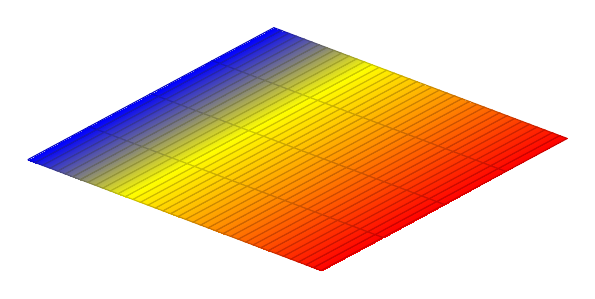
\begin{tikzpicture}
					\begin{axis}[
					hide axis,
					view={40}{40}
					]
					\addplot3 [
					surf, shader=faceted interp,
					point meta=x,
					samples=40,
					samples y=5,
					z buffer=sort,
					domain=0:360,
					y domain=-0.5:0.5
					] (
					{x},
					{y},
					{0});
					\end{axis}
				\end{tikzpicture}
				$M:ax_1+bx_2+cx_3=d\\
				U:=(a,b,c)$ constant.\\
				$\forall p \in M, S(\vec{v})=-\nabla_{\vec{v}}U=(0,0,0)$.
			\item Sphere: 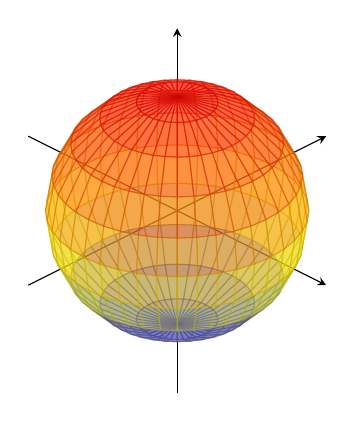
\begin{tikzpicture}
					\begin{axis}[%
					axis equal,
					width=10cm,
					height=10cm,
					axis lines = center,
					ticks=none,
					enlargelimits=0.3,
					view/h=45,
					scale uniformly strategy=units only,
					]
					\addplot3[%
					opacity = 0.5,
					surf,
					z buffer = sort,
					samples = 21,
					variable = \u,
					variable y = \v,
					domain = 0:180,
					y domain = 0:360,
					]
					({cos(u)*sin(v)}, {sin(u)*sin(v)}, {cos(v)});
					\end{axis}
				\end{tikzpicture}\\
				$S^2(r):=\{\vec{x} \in \R^3:\abs{\vec{x}}=r \}$
				Set $U(\vec{x})=\frac{1}{r}(x_1,x_2,x_3)\\
				\forall p \in S^2(r), \vec{v} \in T_p(s^3(r)),\\
				S_p(\vec{v})=-\nabla_{\vec{v}}U=-\frac{1}{r}\nabla_{\vec{v}}(\vec{x})\\
				=\frac{1}{r}\sum_{i=1}^{3}(\vec{v}[x_i])e_i=-\frac{1}{r}\vec{v}$
%				
				\item $M:=$ cylinder in $\R^3$ given by $x_2^2+x_3^2=r^2\\
				U(\vec{x})=(0,\frac{x_2}{2},\frac{x_3}{r})\\
				p=(0,0,r)$.\\
				(Any $\vec{v}\in T_pM$ has form $v_1\vec{e_1}+v_2\vec{e_2})$\\
				Set $S_{\vec{e_1}}=0,$since $U \equiv (0,0,1)$ here.\\
				$S_{\vec{e_2}}(U)=-\frac{1}{r}(\vec{e_2})$.\\
				Thus, $S_{\vec{v}}(U)=v_1 S_{\vec{e_1}}(U)+v_2 S_{\vec{e_2}}(U)$.\\
				$S_{\vec{v}}(U)=(0,\frac{-v_2}{r},0)$.
				\item Saddle: \textbf{Missing}
			\end{enumerate}
	\end{example}

	\section*{Lecture 2019.11.21}
	$p \in M \subset \R^3$ (surface).\\
	$U$, locally specified unit normal vector field near $p$.\\
	Recall \begin{align*}
	S_{(p)}:T_pM& \to T_pM\\
	\vec{v} &\to -\nabla_{\vec{v}}U
	\end{align*}
	(Shape operator)\\
	Last day:\\
	$K(p):= \det S_{(p)}$ (Gaussian curvature)\\
	$H(p):= \frac{1}{2} ... $ \textbf{Some other curvature?}\\
	Note $\abs{\vec{v}}=1$, so there is a "circle" of slice places, slice curves.\\
	Let $T_{\vec{v}}$ and $N_{\vec{v}}$ denote the tangent and normal vector fields along $\alpha_{\vec{v}}$.\\
	\textbf{Fact:} The curve $\alpha_{\vec{v}}$ is planar (by construction) ($\tau \equiv 0$).\\
	In particular, $N(=N_{\vec{v})}= \pm U \mid_{\alpha_{\vec{v}}}$ (along $\alpha_{\vec{v}})$).\\
	Thus, \[\nabla_{\vec{v}}N=\pm S(\vec{v}) = - \nabla_{\vec{v}}U \] $\nabla_{\vec{v}}N=\nabla_{\alpha'(0)}N$ where $\alpha=\alpha(s)$ unit speed parametisation and $s \in (-\epsilon,\epsilon)$ and $\alpha(0)=p$.\\
	But $\nabla_{\alpha'(0)}N=N'(0)=-\kappa(0)T(0) \underbrace{+0}_{T \equiv 0}$\\
	Observe that $\abs{\kappa(0))}=\frac{1}{r_v}$ where $r_v=$ radius of the oscillating circle to $\alpha_v$ at $p$.\\
	Let $S'(T_pM) := \{ \vec{v} \in T_pM:\abs{\vec{v}}=1\}$\\
	Restrict $S_p:S'(T_pM) \to T_pM$\\
	As $S'(T_pM)$ is compact (closed and bounded) in $T_pM$ we know that the corresponding curvature attains maxima and minima.\\
	Fact from linear algebra: $\vec{v}_{\min}$ and $\vec{v}_{\max}$ are eigenvectors of $S_p$ and $\kappa_{\min}$ and $\kappa_max$ are the corresponding eigenvalues.\\
	Thus $K(P)=\kappa_max \kappa_{\min}$\\
	$H(p)=\frac{1}{2}(\kappa_max+\kappa_{\min})$.\\
	\\
	Back to yesterday's examples:\\
	\begin{enumerate}
		\item $S^2(r), S_p(\vec{v})=-\frac{1}{r} \vec{v}$\\
		\[S_p= \begin{bmatrix}
			-\frac{1}{r} & 0\\
			0 & -\frac{1}{r}
		\end{bmatrix} \]
		$\kappa_{\min} = \kappa_{\max}=-\frac{1}{r}$\\
		$K(p)=\frac{1}{r^2}>0\\
		H(p)=-\frac{2}{r}$
		\item Cylinder $y^2+z^2=r^2$\\
		$S(\vec{v})=-\frac{1}{r}v_2$ \[ S=\begin{bmatrix}
			0 & 0 \\
			0 & -\frac{1}{r}
		\end{bmatrix} \]
		$k_{\min} = -\frac{1}{r}, k_{\max} = 0\\
		k=0,H=-\frac{1}{2r}$
		\item Graph of $f(x,y)=xy$,\\
		$p=(0,0,0)\\
		S_p(\vec{e_1})=\vec{e_1}\\
		S_p(\vec{e_2})=\vec{e_1}$
		\[ S_p = \begin{bmatrix}
			0 & 1\\
			1 & 0
		\end{bmatrix} \]
	\end{enumerate}

	\section*{Lecture 2019.11.27}
	\textbf{Correction:}\\
	$p \in M \subset \R^3$ surface. $U$ unit normal vector field near $p$. $\vec{v} \in T_pM$, $\abs{\vec{v}}=1$.\\
	$\alpha$ arbitrary (regular unit speed) curve: $\alpha(0)=p$, $\alpha'(0)=v$.\\
	\textbf{Fact:}\\
	$\alpha'.U \equiv 0$.\\
	$\dv{}{t}\left(\alpha'.U\right)=0$. Thus $\alpha''.U=-\alpha'.U$.\\
	Consider the shape operator:\\
	\textbf{Missing!}\\
	Now consider $S(\vec{v}).\vec{v}$. \begin{align*}
		S(\vec{v}).\vec{v}&=-U'(0).\alpha'(0)\\
		&=-\left(-\alpha''(0).U(p)\right)\\
		&=\alpha''(0).U(p)\\
		&=\abs{\alpha''(0)}N_\alpha(0).U(p) & (\mathrm{assume} \ \alpha''(0) \neq 0)\\
		&=\underline{\kappa_\alpha(0)}\ \underline{N_\alpha(0).U(p)}\\
		&=\kappa_\alpha(0).\cos\theta
	\end{align*}
	Now assume $\alpha$ is a slicing curve given by the slice plane spanned by $\vec{v}$ and $U(p)$.\\
	In this case $\cos \theta= \pm 1$.\\
	Now consider the function ($S$ is unit tangent vectors) \begin{align*}
		S(T_pM)&\to\R\\
		\vec{v}& \mapsto S(\vec{v}).\vec{v} & = \pm \kappa_{\vec{v}}(0)
	\end{align*}
	Curvature of slicing curve through $\vec{v}$.\\
	This attains max, min:
	\begin{align*}
		v_{\min}&\mapsto k \min(p)\\
		v_{\max}&\mapsto k \max(p)
	\end{align*}
	from eigenvectors of $S$ to eigenvalues of $S$.\\
	\textbf{Missing...}
	
	\section*{Geodesic Triangles}
	Recall \begin{align}
		S^2(r) & \qquad k \equiv \frac{1}{r^2}\\
		\mathrm{Plane} & \qquad k \equiv 0\\
		\mathrm{Saddle} & \qquad k < 0
	\end{align}
	\begin{enumerate}
		\item Geodesics converge, $\alpha+\beta+\gamma>\pi$.
		\item Geodesics diverge at a constant rate, $\alpha+\beta+\gamma=\pi$.
		\item Geodesics diverge rapidly, $\alpha+\beta+\gamma<\pi$
	\end{enumerate}
	Consider $S^2(1)$. Pick 3 points, make triangle using great circles.\\
	Any 2 of these great circles forms a \textbf{'lune'}.\\
	$\alpha-lune$, Area($\alpha-$lune)=$4 \alpha$.
	
	\section*{Lecture 2019.11.28}
	\textbf{Geodesics (ctd.)}\\
	2 classical observations:
	\begin{enumerate}
		\item Geodesics on a plane are precisely straight lines.
		\item Geodesics on the sphere are precisely great circles (or segments of the circles).
	\end{enumerate}

	\begin{proof}[Proof of (1)]
		Suppose $\alpha$ is a straight line on a plane $P$.\\
		Figure is plane, line diagonal, arrows pointing up from plane. $p \subset \R^3$.\\
		$p:ax+by+cz=d\\
		\vec{n}=(a,b,c)$
		Thus $\alpha'(t)=a\\
		\alpha''(t)=\vec{0} \perp P.$\\
		\textbf{Missing a line...}\\\
		Now suppose $\alpha$ is a geodesic on $P$. Notice \qquad \begin{align*}
			\alpha'.U&\equiv 0\\
			\alpha''.U+\alpha'.U'&=0
		\end{align*}
		\textbf{Might be missing something?}
		As $U$ constant, $\alpha''.U=0$\\
		As $\alpha''$ both $\parallel$ and $\perp$ to $U$, $\alpha''=\vec{0}$.\\
		Thus $\begin{aligned}
			\alpha'(t)&=\vec{a}\\
			\alpha(t)&=\vec{a}t+b
		\end{aligned}$
	\end{proof}

	\begin{proof}[Proof of (2)]
		Suppose $\alpha$ is a great circle on $S^2(r)$. Then, $\alpha''$ is inward pointing (to original) normal vector field. Thus $\alpha$ is a geodesic.\\
		Now suppose $\alpha$ is a geodesic on $S^2(r)$. We must show $\alpha$ forms part of a great circle.\\
		\textbf{Ingredients:}
		\begin{enumerate}
			\item Consider a curve $\alpha$ on $S^2(r)$.
			\textbf{Claim:} $\alpha$ has everywhere non-zero curvature.\\
			Assume $\alpha$ unit speed etc.\\
			\begin{align*}
				\alpha.\alpha&=r\\
				\alpha'.\alpha&=0\\
				\alpha''.\alpha+\alpha'.\alpha'&=0\\
				\alpha''.\alpha&=-T.T=-1
			\end{align*}
			Thus $\alpha''(t) \neq (0,0,0)\ \forall t$.\\
			Furthermore \[ \abs{\alpha''.\alpha} = \abs{\kappa N.\alpha} = 1 \quad \mathrm{and} \quad \abs{\kappa N.\alpha} \leq \abs{\kappa N} \abs{\alpha} \leq \kappa r \]
			We have $1 \leq \kappa r$ and so $\kappa \geq \frac{1}{r}$.\\
			Now assume $\alpha$ geodesic on $S^2(r)$.\\
			At any $t,$, \begin{align*}
				S(\alpha'(t))&=-\nabla_{\alpha'(t)}U\\
				&=\nabla_{\alpha'(t)}N\\
				&=N'
			\end{align*} where $U=$ outward unit normal to $S^2(r)$, $N$ is normal to $\alpha$.\\
			Recall $N'=-\kappa T + \tau B$.\\
			\[=-\kappa T+\tau B \]
			\textbf{Missing a good bit of stuff (SIG)}
			
			
				
			
		\end{enumerate}
	\end{proof}

	\section*{Lecture 2019.12.04}
	$p \in M \subset \R^3\\
	U$ loc. unit normal vector field near $p$.
	\begin{align*}
		S:T_pM & \to T_pM\\
		\vec{v}&\mapsto -\nabla_{\vec{v}}U\\
		K(p) &= \det S\\
		H(p) &= \frac12 tr S
	\end{align*}
	\textbf{Missing some stuff (late)}\\
	\textbf{Fact:} One can obtain $k_{\min}$, $k_{\max}$ from $K,H$.
	\begin{proof}
		$\underbrace{\det (S-kI)}_{\mathrm{char.\ poly.} p(k)}=0$ characteristic equation.
		$\begin{matrix}
			S&=&\begin{bmatrix}
			s_{11} & s_{12}\\
			s_{21} & s_{22}
			\end{bmatrix}\\\\
			S-kI &=&\begin{bmatrix}
			s_{11}-k & s_{12}\\
			s_{21} & s_{22} -k
			\end{bmatrix}
		\end{matrix}$\\
		\textbf{Missing stuff (he fast)}\\
		Set $p(k)=0$.
		\begin{align*}
			k^2-2Hk_k & = 0\\
			k&=\frac{2H \pm \sqrt{4H^2-4K}}{2}\\
			&=H \pm \sqrt{H^2-k}
		\end{align*}
		Thus $k_{\min}, k_{\max} = H \pm \sqrt{H^2-K}$.
	\end{proof}
	$M \subset \R^3$. We're using a domain $D$ which contains the geometric properties of a curvature in $R^3$. which is \textbf{pulling back the metric}.\\
	As $x$ is a local param u.\\
	\[ x_u(u_0,v_0),x_v(u_0,v_0)\ \mathrm{span}\ T_{x(u_0,v_0)}M\]
	$\forall u_0,v_0$.\\
	We are interested in the behaviour of the frame $\{x_u,x_v\}$ over the domain $D$.\\
	Lots of notation:
	\[\begin{matrix}
		E &=& x_u.x_u &=& \abs{x_u}^2\\
		F &=& x_u.x_v &=& \abs{x_u}\abs{x_v}\cos \theta\\
		G &=& x_v.x_v &=& \abs{x_v}^2
	\end{matrix}\] are scalar functions on $D$.\\
	Thus $F=\sqrt{EG}\cos \theta$.\\
	\[x_u \times x_v = \abs{x_u} \abs{x_v} \sin \theta = \sqrt{EG} \sin \theta \] area of parallelogram.
	\begin{align*}
		\abs{x_u \times x_v}^2 &= EG \sin^2 \theta\\
		&= EG(1-\cos^2\theta)\\
		&=EG(1-\frac{F^2}{EG})\\
		&=EG-F^2\\
		\abs{x_u \times x_v} &= \sqrt{EG-F^2}
	\end{align*}
	Obtain loc. unit normal
	\[U:=\frac{x_u \times x_v}{x_u \times x_v} = \frac{x_u \times x_v}{\sqrt{EG-F^2}}\]
	We have the shaoe io $S$ in terms of $U$.
	\begin{align*}
		l&:=S(x_u).x_u\\
		m&:=S(x_u).x_v\underbrace{=}_{\mathrm{exercise}}S(x_v.x_u)\\
		n&:=S(x_v).x_v
	\end{align*}
	
	\begin{remark}[Aside:]
		3 symmetric bilinear forms:\\
		\[\begin{matrix}
			& T_pM \times T_pM& \to & \R^3\\
			I: & (\vec{v},\vec{w}) & \mapsto & \vec{v}.\vec{w}\\
			II:& (\vec{v},\vec{w}) & \mapsto & S(\vec{v}).\vec{w}&=&S(w).\vec{v}\\
			III:& (\vec{v},\vec{w}) & \mapsto & S(\vec{v}).S(\vec{w})
		\end{matrix}\]
	\end{remark}

	\begin{theorem}
		\begin{align*}
			K&=\frac{ln-m^2}{EG-F^2}\\
			H&=\frac{Gl+En-2Fm}{2(EG-F^2)}
		\end{align*}
		\begin{proof}Long calculation.\end{proof}
		To calculate $l,m,n$ we use the following observation.\\
		Notice $x_u.U\equiv 0$.\\
		\[0=\pdv{}{v}(x_u.U)=x_{uv}.U+x_u.U_v\]
		So \begin{align*}
			x_{uv}.U&=-X_u.U_v\\
			&=-U_v.x_u\\
			&=-(-S(x_v).x_u)\\
			&=S(x_v).x_u\\
			&=m
		\end{align*}
		Using similar arguments:
		\begin{align*}
			l &= x_{uu}.U\\
			m&=x_{uv}.U\\
			n&=x_{vv}.U
		\end{align*}
	\end{theorem}
	\begin{example}[Helicoid]
		$u>-, v \in (0,2 \pi )\\
		x(u,v)=(u \cos v,u \sin v, bu)\ 0<b$ constant.\\
		Ex. Fill in $x_u, x_v, x_{uv}$ etc. 
		\[\begin{matrix}
			E\equiv 1 & F \equiv 0 & G = b^2+u^2\\
			l \equiv 0 & m=\frac{-b}{\sqrt{b^2+u^2}} & n \equiv 0
		\end{matrix}\]
		\[K=\frac{-b^2}{(b^2+u^2)^2}\]
		$H=0$\\
		$-1 < k < 0$.
	\end{example}

	\section*{Lecture 2019.12.05}
	Summary of notation:
	\begin{align*}
		E &= x_u.x_u\\
		F&=x_u.x_v=x_v.x_u\\
		G&=x_v.x_v\\
		\abs{\abs{?}}&=\\
		??\\
		S&=\mathrm{shape\ operator}\\
		l&=S(x_u).x_u = x_{uu}.U\\
		m&=S(x_u).x_v = S(x_v).x_u = x_{uv}.U\\
		n&=S(x_v)\ \ddd ????\\
		K&=\frac{ln-m^2}{EG-F^2}\\
		H&=\frac{Gl+En-2Fm}{2(EG-F^2)}		
	\end{align*}
	\begin{example}[Helicoid example:]
		\[x(u,v)= (u \cos v ,u \sin v, bv),\ u > 0,\ v \in [0,2\pi) \]
		\[K=\frac{-b^2}{(b^2+u^2)^2}\qquad H \equiv 0 \]
	\end{example}
	\begin{example}[Saddle example:]
		\[x:(u,v) \mapsto (u,v,uv)\]
		\[ K=\frac{-1}{(1+\underbrace{u^2+v^2}_{r=\sqrt{u^2+v^2}})^2} \qquad H=\frac{-uv}{(1+u^2+v^2)^{\frac{3}{2}}}\]
	\end{example}

	\begin{remark}[Technical Fact:]
		Assume $x_u \perp x_v$. i.e. $F \equiv 0$.
		\begin{align*}
			S(x_u)&=\left(S(x_u).\frac{x_u}{\abs{x_u}}\right)+\left(S(x_u).\frac{x_v}{\abs{u_v}}\right)\frac{x_v}{\abs{x_v}}\\
			&= \left(\frac{l}{E}\right)x_u+\left(\frac{m}{G}\right)x_v\\
			S(x_v)&=\left(\frac{m}{E}\right)x_u+\left(\frac{n}{G}\right)x_v
		\end{align*}
	\end{remark}
	\begin{example}[Rotationally symmetric surfaces]
		Start with curve $u \mapsto (g(u),h(u))$ in $x-y$ plane.\\
		Rotate about $x$-axis.\\
		Surface of revolution given by \[x(u,v)=\left(g(u),h(u)\cos v, h(u)\sin v\right),\qquad u \in \R, v \in [0,2\pi)\]
		Curvature calculation (highlights):
		\begin{align*}
			x_u &= \left(g'(u),h'(u) \cos v, h'(u) \sin v\right)\\
			x_v &= \left(0,-h(u)\sin v, h(u) \cos v \right)\\
			E&=(g')^2+(h')^2\\
			F & \equiv 0\\
			G = h^2\\
			\abs{x_u \times x_v} &= \sqrt{EG-F^2}\\
			&= \sqrt{h^2[(g')^2+(h')^2]}\\
			&=h\sqrt{(g')^2+(h')^2}\\
			x_u \times x_v &= \left( hh',-hg'\cos v, -h g' \sin v \right)
		\end{align*}
		Compute $x_{uu},x_{uv},x{vv}$ to obtain \begin{align*}
			l&=\frac{\left(-g'h''+g''h'\right)}{\sqrt{(g')^2+(h')^2}}\\
			n&=\frac{g'h}{\sqrt{(g')^2+(h')^2}}
			m&=0\\
		\end{align*}
		Earlier technical fact (with $m=0$) gives:
		\begin{align*}
			S(x_u)&=\frac{l}{E}x_u\\
			S(x_v)&=\frac{n}{G}x_v
		\end{align*}
		Thus principal curvatures are $\frac{l}{E}$ and $\frac{n}{G}$.\\
		So \[K=\frac{l}{E}.\frac{n}{G},\qquad H=\frac{1}{2}\left(\frac{l}{E}+\frac{n}{G}\right) \]
		\begin{align*}
			K&=\left(\frac{\left(\frac{-\det \begin{bmatrix}
				g' & h'\\
				g'' & h''
			\end{bmatrix}}{\sqrt{(g')^2+(h')^2}}\right)}{((g')^2+(h')^2)}\right)
			\left(\frac{\frac{g'h}{\sqrt{(g')^2+(h')^2}}}{h^2}\right)
			\\
		\end{align*}
		
		
	\end{example}
	\begin{example}
		\[x(u,v)=\left((R+r\cos u)\cos v, (R+r\cos u)\sin v, \sin u\right)\]
		Principal curvatures : $\frac1r,\frac{\cos u}{(R + \cos)}$\\
		\textbf{Missing the end...}\\
	\end{example}

	\section*{Lecture 2019.12.11}
	\textbf{Missing beginning (bike puncture)}\\
	Princ. curves for Catenoid:
	\begin{align*}
		h(u)&=b \cosh \frac{u}{b}\\
		h'(u)&=\sinh \frac{u}{b}\\
		h''(u)&=\frac{1}{b}\cosh \frac{u}{b}\\
		\\k_1&=\frac{-\frac{1}{b}\cosh\frac{u}{b}}{\left(1+\sinh^2\frac{u}{b}\right)^\frac{3}{2}}\\
		&=\frac{-\frac1b\cosh\frac{u}{b}}{\cosh^2\frac{u}{b}}\\
		&=-\frac{1}{b \cosh^2 \frac{u}{b}} & \mathrm{Check\ this\ line}\\
		\\
		K&=-\frac{1}{b^2\cosh^4 \frac{u}{b}} & = k_1k_2	
	\end{align*}
	Case when $b=1$, $-1 \leq K < 0$.\\
	\\
	\begin{remark}
		\textbf{Fact: }Helicoid, Catenoid ($b=1$ both cases) are \textbf{locally isometric} surfaces.\\
		\textbf{Idea: }Consider plane and cylinder. Intrinsic geometry is the same even though differently embedded in $\R^3$. These are \textbf{isometric}.\\
	\end{remark}

	\begin{definition}[Local Isometry]
		Suppose $M_1, M_2$ are surfaces in $\R^3$. A smooth function $F:M_1\to M_2$ is a \textbf{local isometry} if $\forall p \in M,\ \vec{v},\vec{w} \in T_pM$, the deriviative map $Df_p:T_pM_1 \to T_{f(p)}M_2$ satisfies $Df_p(\vec{v}).Df_p(\vec{w})=\vec{v}.\vec{w}$.
	\end{definition}

	\begin{remark}[Exercise]\ \\
		Show that $f$ preserves (locally) distance and angle.
	\end{remark}

	\begin{definition}[Isometry]
		If $f$ is also a diffeomorphism we say $f$ is an \textbf{isometry}.
	\end{definition}

	\begin{example}[Plane to Cylinder]
		We use the map \[ f(u,v)=\left(u,r\cos\frac{v}{r},r\sin\frac{v}{r}\right) \]
	\end{example}

	\begin{example}
		Prev catenoid: \[g(u)=u,\quad h(u)=\cosh u\]
		New catenoid:
		\[\begin{matrix}
			g(u)=\sinh^{-1}u & \cosh^2t-\sinh^2=1\\
			h(u)=\sqrt{1+u^2} & \cosh^2t=\sqrt{1+\sinh^2}
		\end{matrix}\]
	\end{example}

	\section*{Lecture 2019.12.18}
	Let $M$ be  2-dim manifold.\\
	Not necessarily embedded in $\R^3$ (intrinsic).\\
	We want to provide a grometric classification of 2-manifolds.\\
	Example: $S^2$. Can be "squished" to be topologically the same, geometrically different.\\
	Example: Torus\\
	Flat torus $\not\subset \R^3$ (can't be embedded).\\
	Want (1) topological  classification e.g. distinguishes $S^2$ from $T^2$ etc. and (2) a "best" geometry in each case.\\
	Topological classification of 2-manifolds:
	\begin{enumerate}
		\item Orientable: $S^2, T^2, T^2 \underbrace{\#}_\mathrm{connected\ sum} T^2 \ddd T^2 \# T^2 \# \ddd \# T^2\ m$ times.\\
		$X,Y$ surfaCes, $X \# Y$ obtained by fluing $X \backslash D^2$ to $Y \backslash D^2$.
		\item Non-orientable: $\R p^2 \cong \mathrm{M\ddot{o}}$.\\
		\textbf{Missing stuff}
	\end{enumerate}
	\begin{theorem}[Uniformisation Theorem]
		Every 2-dim (cpt.) manifold admits a constant (Gaussian) curvature geometry.
	\end{theorem}
	Examples: $S^2(r)$ (round geometry),\ $K \equiv \frac1{r^2},\quad k \equiv 1\\
	T^2\quad K \equiv 0$ (flat torus.)
	
	For $\R p^2$ (pacman), we can increase curvature uniformly. We can make it locally round. Angle arond vertex < $2 \pi $.\\
	We make angle aroudn pt. to be $2 \pi$\\
	\\
	What about $\#$ sum of tori. $T^2 \# T^2$. Merge squares with arrows into isomorphic octagon. Angles around vertex $> 2\pi$ (opposite of cone point).\\
	Ma,e curvature negative.\\
	Squeezes the angles to make them fit.\\
	So we can equip any connected sum of 2+ torii with $K \equiv -1$ geometry...\\
	Also for $\R p^2 \# \R p^2 \# \ddd \# \R p^2$, 3+ pacman thingies.\\
	At this stage have shown \[\begin{matrix}
		S^2,\R p^2 & K \equiv 1\\
		T^2,Kl^2 & \mathrm{admit} & K \equiv 0\\
		\mathrm{else} & \mathrm{admit} & \equiv -1
	\end{matrix}\]
	
	\section*{Lecture 2019.12.19}
	\theoremstyle{Gauss-Bennett Theorem}
	\[\frac{1}{2\pi} \int_M k \d A = \chi (M)  \]
\end{document}
